\documentclass{jarticle}
\usepackage{robomech2022}
\usepackage[dvipdfmx]{graphicx}

\begin{document}
\makeatletter
\title{視覚と行動のend-to-end学習により経路追従行動をオンラインで\\模倣する手法の提案}
{―経路への復帰行動の解析と復帰行動を強化する教師データ収集法の検討―}
{A proposal for an online imitation method of
path-tracking behavior by end-to-end\\ learning of vision and action}
{-Analysis of return-to-pathway behavior and
a method of collecting training data to
enhance\\ return-to-pathway behavior-}

\author{
\begin{tabular}{ll}
 \hspace{1zw}○学\hspace{1zw}今井悠月 (千葉工大)&\hspace{1zw}学\hspace{1zw} 清岡優祐(千葉工大)\\
 \hspace{1zw}\hspace{1zw}正\hspace{1zw}上田隆一 (千葉工大)&\hspace{1zw}正\hspace{1zw} 林原靖男(千葉工大)\\
 % ※協賛・後援団体の会員資格で発表される場合は「正・学」は不要です。
 &\\
 \multicolumn{2}{l}{\small Yuzuki IMAI, Chiba Institute of Technology, s20c1015as@s.chibakoudai.jp}\\
 \multicolumn{2}{l}{\small Yusuke KIYOOKA, }\\
 \multicolumn{2}{l}{\small Ryuichi UEDA and Yasuo HAYASHIBARA, Institute of Technology}\\
\end{tabular}
}
\makeatother

\abstract{ \small 
We have proposed an online imitation method of path-following behavior based on end-to-end learning of vision and action.
In recent years, many studies of atonomous movement using end-to-end learning have been reported, but these studies have also observed deviations from the target path.
One of the possible reasons for this is the lack of training data for returning to the path.
In this paper, we perform end-to-end learning to follow a route generated by a map-based navigation system. The dataset was collected in two ways, one is to learn only the area around the route and the other is to learn the state away from the route, and the generated route-following behaviors were analyzed.
In addition, we proposed a new method of collecting teacher data to reinforce the behavior of returning to the path, and verified the effectiveness of the method by experiments using a simulator.
}

\date{} % 日付を出力しない
\keywords{atonomous movement, navigation, end-to-end learning, dataset}

\maketitle
\thispagestyle{empty}
\pagestyle{empty}

\small
\section{緒言}%===========================本文:明朝体・9pt(欧文Times New Roman, 9pt)、文字間隔は1行26文字程度、行間隔は4.2mm程度にして下さい。
我々は, 入出力関係を直接学習する end-to-end 学習器により,
人の操作ではなく, 地図ベースのナビゲーションシステムを用いた
経路追従行動を視覚に基づいてオンラインで模倣する手法を提案し,
その有効性を実験により検証してきた[1][2].

地図ベースのナビゲーションとは, LiDAR や IMU, ホイールオドメトリなど複数のセンサから占有格子地図を作成し, その地図
を用いて自己位置推定, 経路計画, 制御などの複数のタスクを達成することで目的となる場所
へ自律的に移動する手法である[3].

近年, 画像を入力とした end-to-end 学習による自律移動手法が注目されている.
例えば, Muller らは, 人が操作したコントローラ操作を教師データとして学習することで, 
オフロード環境で障害物を回避しながら走行できることを確認した[4].
また, Bojarski らは画像と人が操作した制御コマンドを end-to-end 学習するこ
とで,自動車を対象とした自律移動手法を提案した[5].

しかし, それらの研究では必ずしも学習した経路を追従できる
わけではなく, 目標とする経路から外れていく様子が確認されている.
その要因の一つとして, 目標となる経路からズレが生じた際
に訓練データにない状態に陥り, 目標となる経路への復帰ができなくなったことが考えられる.
すなわち経路へ復帰するための学習データが不足していることが考えられる.

そこで本稿では, カメラ画像を入力とした end-to-end 学習による自律移動手法において, 図1に示すような
常に経路周辺を学習する場合と, 図2に示すような目標経路周辺だけでなく目標経路から離れた状態も学習する場合の
二つの方法でデータセットを収集し, 学習を行う.[6] そして, その学習によって生成された経路追従行動を分析
を行い, 離れた状態からの復帰行動を学習することが, 有効であることを明らかにする. それに加え, 
目標経路への復帰行動を強化する教師データ収集法を新たに提案し, 有効性を検証する.


\begin{figure}[h!]
  \centering
   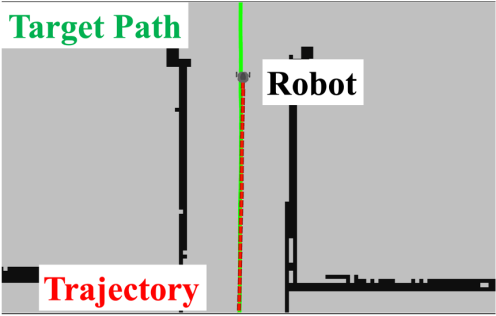
\includegraphics[height=34mm]{./figs/only.png}
   \vspace*{-5mm}
   \caption{Learning only around the target path}
\end{figure}

\begin{figure}[h!]
  \centering
   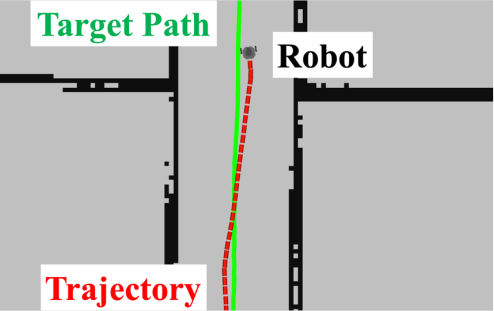
\includegraphics[height=34mm]{./figs/outof.png}
   \vspace*{-5mm}
   \caption{Learning also for states away from the target path}
\end{figure}

 
\section{地図ベースのナビゲーションをオンラインで模倣する手法}
地図ベースのナビゲーションをオンラインで模倣する手法の概要を以下に示す.
この手法は, 地図ベースのナビゲーションシステムの出力である角速度を教師データとして学習し, 
その後, 画像を入力とした学習器の出力によってロボットを制御する. 本稿では, 
地図ベースのナビゲーション教師データとして学習する段階を学習フェーズとし, 学習器の出
力でロボットが自律移動できるかテストする段階をテストフェーズとする.

\subsection{学習フェイズ}
図3に学習フェーズのシステムの概要を示す. 学習フェーズでは地図ベースのナビ
ゲーションを利用することで, ロボットは自律移動を行う. それと同時に, 画像と地図ベー
スのナビゲーションシステムから出力される目標角速度をペアにしたデータセットを収集し, 
end-to-end 学習を行う.
地図ベースのナビゲーションは LiDAR とオドメトリを入力とするのに対し, 学習器は画像
を入力とする. 本手法を用いて学習することで, LiDAR, オドメトリを使用した時と同じ行
動を, 画像のみで行うことが期待できる. なお他の研究に倣い, 3台のカメラを用いて学習を
行う [5][7]. この時, 表1に示すように左右のカメラにオフセットを加え,データセッ
トに与えることでデータの量を増やすことに加え,過学習を防ぐ効果が期待できる.画像は
64 x 48 にリサイズして使用する.ロボットを制御するためのモジュールは navigation[8] と
学習器の二つで構成されており,この二つを切り替えることが可能となっている.

\begin{figure}[h!]
  \centering
   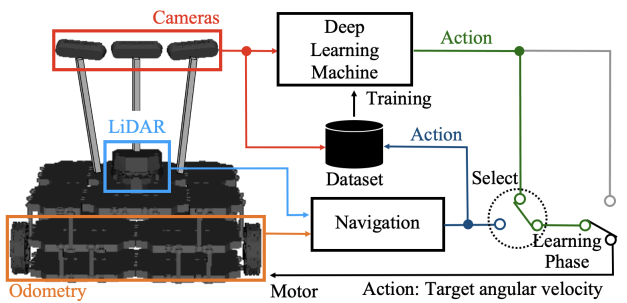
\includegraphics[height=42mm]{./figs/learning.png}
   \vspace*{-4mm}
   \caption{Learning phase}
\end{figure}


\begin{table}[htbp]
  \caption{: Three cameras and data to be labeled} \vspace*{3mm}
  \hspace*{-7mm}
  \begingroup
    \renewcommand{\arraystretch}{1.2}
    \begin{tabular}{|l|l|}
      \hline
      Cameras & Labelling data [rad/s] \\
      \hline
      Left camera & Map-based navigation system output + 0.2 \\
      Center camera & Map-based navigation system output \\
      Right camera & Map-based navigation system output - 0.2 \\
      \hline
    \end{tabular}
  \endgroup
\end {table}


\subsection{テストフェイズ}
テストフェーズでは, Fig. 3.4 のように学習フェーズで学習したモデルを用いてロボット
を制御し, 律移動できるかテストする. 64x48 にリサイズした画像を学習器に入力し, の
推定結果をロボットの目標角速度としてロボットを自律移動させる.ロボットの角速度は学習
器の出力を用いるが, 進速度は学習フェーズと同様に一定 (0.2m/s) とする.なお, スト
フェーズでは3台のカメラのうち, 央のカメラのみ使用する.

\begin{figure}[h!]
  \centering
   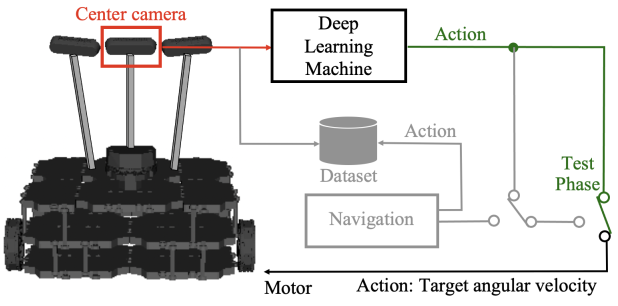
\includegraphics[height=42mm]{./figs/test.png}
   \vspace*{-4mm}
   \caption{Test phase}
\end{figure}


\footnotesize
\begin{thebibliography}{99}

\bibitem{1}
岡田眞也, 清岡優祐, 上田隆一, 林原靖男: “視覚と行動の end-
to-end 学習により経路追従行動 をオンラインで模倣する手法
の提案”, 計測自動制御学会 SI 部門講演会 SICE-SI2020 予稿
集, pp.1147-1152(2020).

\bibitem{2}
岡田眞也, 清岡優祐, 春山健太, 上田隆一, 林原靖男:“視覚と
行動の end-to-end 学習により経路追従行動 をオンラインで
模倣する手法の提案 -経路追従行動の修正のためにデータセッ
トを動的に追加する手法の検討”, 計測自動制御学会 SI 部門
講演会 SICE-SI2021 予稿集, pp.1066-1070(2021).

\bibitem{3}
W. Schwarting, J. Alonso-Mora, and D. Rus.
Planning and decision making for
autonomous vehicles . Annu. Rev, Vol. 1, No. 1, pp. 187-210, May 2018.

\bibitem{4}
U. Muller, J. Ben, E. Cosatto, B. Flepp, and Y. Cun. ”Off-road obstacle avoidance
through end-to-end learning”. Advances in neural information processing systems,
Vol. 18, , 2005.

\bibitem{5}
Bojarski, Mariusz, and et al.
"End to end learning for self-driving cars".
arXiv:1604.07316, 2016.

\bibitem{6}
清岡優祐 , 岡田眞也 , 岩井一輝 , 上田隆一 , 林原靖男 .
より経路追従行動をオンラインで模倣する手法の提案
視覚と行動の end-to-end 学習に
ー データセットと生成された
経路追従行動の解析 ー . 計測自動 制御学会 SI 部門講演会 SICE-SI2021 予稿集 , pp.1071-1075, 2021.

\bibitem{7}
Moridian, Barzin, Anurag Kamal, and Nina Mahmoudian.
Learning navigation
tasks from demonstration for semi-autonomous remote operation of mobile robots .
IEEE International Symposium on Safety, Security, and Rescue Robotics (SSRR),
2018.

\bibitem{8}
ros-planning, navigation リポジトリ ( 最終閲覧日 :2023年 2月6日 ). https://
github.com/ros-planning/navigation.

\end{thebibliography}

\normalsize
\end{document}
